\chapter{बिंदु की शुद्धगतिकी}\label{ch:b1:point-kinematics}

झूला-रेलगाड़ी की डिब्बी \qty{90}{km/h} पर पाश में घुसती है, चढ़ते हुए धीमी
पड़ती है, शिखर पर एक क्षण को ठहरी-सी रहती है, और फिर गरजती हुई निकल जाती है;
उसमें बैठे लोग तल पर सीट में दबे हुए और शिखर पर लगभग भारहीन अनुभव करते हैं।
उस सवारी का वर्णन --- डिब्बी कहाँ है, कितनी तेज़ चलती है, उसका \omterm{def:b1:point-kinematics:velocity}{वेग} किस तरह
मुड़ता और बदलता है --- शुद्धगतिकी है, और इसके लिए सीधी सड़क वाले $x$, $y$,
$z$ से कहीं अधिक चाहिए: जो कुछ घूमता है उसके लिए \omterm{def:b1:point-kinematics:cylindrical}{ध्रुवीय निर्देशांक}, और
स्वयं डिब्बी के साथ चलता हुआ एक आधार। यह अध्याय वही औज़ार जुटाता है, उनमें
से हर एक में \omterm{def:b1:point-kinematics:velocity}{वेग} और \omterm{def:b1:point-kinematics:velocity}{त्वरण} के सूत्र सिद्ध करता है, और उन्हें उन गतियों पर
लगाता है जिन्हें आगे का हर अध्याय बुलाएगा: वृत्तीय, कुंडलिनी, आवर्त, और किसी
भी वक्र के अनुदिश गति।

\section{स्थिति, वेग और त्वरण}

\begin{definition}[निर्देश तंत्र; स्थिति; गतिपथ]\label{def:b1:point-kinematics:frame}
\index{निर्देश तंत्र}\index{स्थिति सदिश}\index{गतिपथ}\index{बिंदु कण}
\emph{निर्देश तंत्र} कोई दृढ़ पिंड है जिसे स्थिर मान लिया जाता है
(प्रयोगशाला, पृथ्वी, कोई रेलगाड़ी), और उसके साथ एक घड़ी। \emph{बिंदु कण}
$M$ --- ऐसा पिंड जिसका आकार अध्ययन की जा रही गति के लिए महत्वहीन हो --- हर
क्षण अपने \emph{स्थिति सदिश} $\vect{OM}(t)$ से नियत होता है, जो तंत्र से जुड़े
किसी मूल बिंदु $O$ से खींचा जाता है; $M$ जो वक्र खींचता है वही उसका
\emph{गतिपथ} है। गति सदा \emph{किसी तंत्र के सापेक्ष} गति होती है: वही यात्री
रेलगाड़ी में विराम में है और स्टेशन में गतिमान।
\end{definition}

\begin{definition}[वेग और त्वरण]\label{def:b1:point-kinematics:velocity}
\index{वेग}\index{त्वरण}
तंत्र में $M$ के \emph{वेग} और \emph{त्वरण} हैं
\[
\vect v = \frac{\dd\vect{OM}}{\dd t}, \qquad
\vect a = \frac{\dd\vect v}{\dd t} = \frac{\dd^2\vect{OM}}{\dd t^2},
\]
जो सदिश फलनों के अवकलज हैं: किसी सदिश का अवकलज उसके घटकों को ऐसे आधार में
अवकलित करके मिलता है जो \emph{तंत्र में स्थिर} हो। वेग \omterm{def:b1:point-kinematics:frame}{गतिपथ} की स्पर्शरेखा
के अनुदिश होता है और गति की दिशा में इंगित करता है; उसका परिमाण $v$
\emph{चाल} कहलाता है। मात्रक: \unit{m/s}, \unit{m/s^2}।
\end{definition}

\begin{proposition}[कार्तीय निर्देशांक]\label{prop:b1:point-kinematics:cartesian}
\index{कार्तीय निर्देशांक}
किसी स्थिर लांबिक-प्रसामान्य आधार $(\vect e_x, \vect e_y, \vect e_z)$ और
$\vect{OM} = x\,\vect e_x + y\,\vect e_y + z\,\vect e_z$ के साथ,
\[
\vect v = \dot x\,\vect e_x + \dot y\,\vect e_y + \dot z\,\vect e_z, \qquad
\vect a = \ddot x\,\vect e_x + \ddot y\,\vect e_y + \ddot z\,\vect e_z,
\]
जहाँ बिंदु $\dd/\dd t$ को दर्शाता है।
\end{proposition}

\begin{proof}
आधार सदिश अचर हैं; केवल घटक बदलते हैं।
\end{proof}

\begin{example}[प्रक्षेप्य]\label{ex:b1:point-kinematics:projectile}
$O$ से चाल $v_0$ और क्षैतिज से $\alpha$ कोण पर फेंकी गई किसी गेंद के
निर्देशांक (गतिकी, अगला अध्याय) हैं
$x = v_0\cos\alpha\,t$, $z = v_0\sin\alpha\,t - \tfrac12 gt^2$। तब
$\vect v = v_0\cos\alpha\,\vect e_x + (v_0\sin\alpha - gt)\vect e_z$,
$\vect a = -g\vect e_z$: \omterm{def:b1:point-kinematics:velocity}{त्वरण} अचर रहता है जबकि \omterm{def:b1:point-kinematics:velocity}{वेग} मुड़ता जाता है; शिखर पर
($\dot z = 0$, $t = v_0\sin\alpha/g$) \omterm{def:b1:point-kinematics:velocity}{वेग} क्षैतिज होता है और \omterm{def:b1:point-kinematics:velocity}{त्वरण} उस पर
लंब। $t$ का लोप करने पर: $z = x\tan\alpha - gx^2/(2v_0^2\cos^2\alpha)$, यानी
एक परवलय।
\end{example}

\begin{omfigure}
\begin{tikzpicture}[font=\small, x=1cm, y=1cm]
  \draw[-Stealth] (0,0) -- (6.8,0) node[right] {$x$};
  \draw[-Stealth] (0,0) -- (0,3.6) node[above] {$z$};
  \node[below left] at (0,0) {$O$};
  \draw[omDef, thick, domain=0:6, samples=80] plot (\x, {2.2*\x - 0.3667*\x*\x});
  % point at x=1.5: z=2.2*1.5-0.3667*2.25=3.3-0.825=2.475 ; slope = 2.2 - 0.7333*1.5 = 1.1
  \fill[omThm] (1.5,2.475) circle (1.6pt); \node[above left] at (1.5,2.475) {$M$};
  \draw[-Stealth, omThm, thick] (1.5,2.475) -- ++(1.0,1.1) node[above right] {$\vect v$};
  \draw[-Stealth, omProp, thick] (1.5,2.475) -- ++(0,-1.2) node[right] {$\vect a = \vect g$};
  \draw[-Stealth, omExo] (0,0) -- (1.5,2.475); \node[omExo, left] at (0.72,1.45) {$\vect{OM}$};
  % apex at x=3: z=6.6-3.3=3.3
  \fill[omThm] (3,3.3) circle (1.6pt);
  \draw[-Stealth, omThm, thick] (3,3.3) -- ++(1.2,0);
  \draw[-Stealth, omProp, thick] (3,3.3) -- ++(0,-1.2);
\end{tikzpicture}

{\small प्रक्षेप्य का परवलय: \omterm{def:b1:point-kinematics:velocity}{वेग} \omterm{def:b1:point-kinematics:frame}{गतिपथ} की स्पर्शरेखा के अनुदिश रहता है और
मुड़ता जाता है, जबकि \omterm{def:b1:point-kinematics:velocity}{त्वरण} $\vect g$ अचर है। शिखर पर \omterm{def:b1:point-kinematics:velocity}{वेग} और \omterm{def:b1:point-kinematics:velocity}{त्वरण} परस्पर लंब
हैं: चाल क्षण भर के लिए ठहरी हुई है, पर दिशा तब भी बदल रही है।}
\end{omfigure}

\section{बेलनाकार निर्देशांक}

\begin{definition}[बेलनाकार निर्देशांक और स्थानीय आधार]\label{def:b1:point-kinematics:cylindrical}
\index{बेलनाकार निर्देशांक}\index{ध्रुवीय निर्देशांक}\index{स्थानीय आधार}
बिंदु $M$ को तीन राशियाँ नियत करती हैं: $r \geq 0$ ($z$ अक्ष से दूरी), कोण
$\theta$, जो $xy$ तल पर उसके प्रक्षेप का $\vect e_x$ से कोण है, और $z$; तब
$\vect{OM} = r\,\vect e_r + z\,\vect e_z$, जहाँ
\[
\vect e_r = \cos\theta\,\vect e_x + \sin\theta\,\vect e_y, \qquad
\vect e_\theta = -\sin\theta\,\vect e_x + \cos\theta\,\vect e_y,
\]
और $\vect e_z$ मिलकर \emph{स्थानीय आधार} $(\vect e_r, \vect e_\theta,
\vect e_z)$ बनाते हैं, जो लांबिक-प्रसामान्य तथा दक्षिणावर्त है और
\emph{$M$ के साथ चलता} है। तल में ($z$ स्थिर) ये \emph{ध्रुवीय निर्देशांक}
$(r, \theta)$ हैं।
\end{definition}

\begin{lemma}[स्थानीय आधार के अवकलज]\label{lem:b1:point-kinematics:basisderiv}
\[
\frac{\dd\vect e_r}{\dd t} = \dot\theta\,\vect e_\theta, \qquad
\frac{\dd\vect e_\theta}{\dd t} = -\dot\theta\,\vect e_r, \qquad
\frac{\dd\vect e_z}{\dd t} = \vect 0 .
\]
\end{lemma}

\begin{proof}
घटकों को अवकलित कीजिए: $\dd\vect e_r/\dd t = \dot\theta(-\sin\theta\,
\vect e_x + \cos\theta\,\vect e_y) = \dot\theta\vect e_\theta$, और इसी तरह
$\vect e_\theta$ के लिए भी। घूमते हुए एकांक सदिश का अवकलज उस पर लंब होता है,
और उसका परिमाण कोणीय दर के बराबर होता है।
\end{proof}

\begin{theorem}[बेलनाकार निर्देशांकों में वेग और त्वरण]\label{thm:b1:point-kinematics:cylindrical}
\[
\vect v = \dot r\,\vect e_r + r\dot\theta\,\vect e_\theta + \dot z\,\vect e_z,
\qquad
\vect a = \big(\ddot r - r\dot\theta^2\big)\vect e_r
+ \big(r\ddot\theta + 2\dot r\dot\theta\big)\vect e_\theta + \ddot z\,\vect e_z .
\]
\end{theorem}

\begin{proof}
प्रमेयिका की सहायता से $\vect{OM} = r\vect e_r + z\vect e_z$ का अवकलन कीजिए:
$\vect v = \dot r\vect e_r + r\dot\theta\vect e_\theta + \dot z\vect e_z$।
फिर से अवकलन कीजिए: $\ddot r\vect e_r + \dot r\dot\theta\vect e_\theta +
\dot r\dot\theta\vect e_\theta + r\ddot\theta\vect e_\theta - r\dot\theta^2
\vect e_r + \ddot z\vect e_z$; अब पदों को इकट्ठा कीजिए।
\end{proof}

\begin{omfigure}
\begin{tikzpicture}[font=\small, x=1cm, y=1cm]
  \draw[-Stealth] (0,0) -- (5.2,0) node[right] {$x$};
  \draw[-Stealth] (0,0) -- (0,3.6) node[above] {$y$};
  \node[below left] at (0,0) {$O$};
  \coordinate (M) at (35:3.4);
  \draw[omExo] (0,0) -- (M); \fill[omThm] (M) circle (1.6pt); \node[below right, xshift=2pt] at (M) {$M$};
  \node[omExo] at (20:1.9) {$r$};
  \draw (0.9,0) arc (0:35:0.9); \node at (17:1.15) {$\theta$};
  \draw[-Stealth, omDef, very thick] (M) -- ++(35:1.1) node[right] {$\vect e_r$};
  \draw[-Stealth, omDef, very thick] (M) -- ++(125:1.0) node[left] {$\vect e_\theta$};
  % trajectory sketch: spiral
  \draw[omThm, thick, domain=5:75, samples=50, variable=\t] plot ({(2.2+0.0343*\t)*cos(\t)},{(2.2+0.0343*\t)*sin(\t)});
  \draw[-Stealth, omThm, thick] (M) -- ++(100:1.6) node[above right] {$\vect v$};
\end{tikzpicture}

{\small \omterm{def:b1:point-kinematics:cylindrical}{ध्रुवीय निर्देशांक}: \omterm{def:b1:point-kinematics:cylindrical}{स्थानीय आधार} $(\vect e_r, \vect e_\theta)$
$M$ के साथ घूमता है; \omterm{def:b1:point-kinematics:velocity}{वेग} में एक त्रिज्य भाग $\dot r$ और एक लंबत्रिज्य भाग
$r\dot\theta$ होता है। यहाँ \omterm{def:b1:point-kinematics:frame}{गतिपथ} (लाल) बाहर की ओर सर्पिल बनाता है, अतः
$\dot r > 0$ है और $\vect v$ वृत्त की स्पर्शरेखा से बाहर की ओर झुका हुआ है।}
\end{omfigure}

\begin{corollary}[वृत्तीय गति]\label{cor:b1:point-kinematics:circular}
\index{वृत्तीय गति}\index{अभिकेंद्र त्वरण}\index{कोणीय वेग}
$R$ त्रिज्या के वृत्त पर ($r = R$, $z = 0$), \emph{\omterm{cor:b1:point-kinematics:circular}{कोणीय वेग}}
$\omega = \dot\theta$ के साथ:
\[
\vect v = R\omega\,\vect e_\theta, \qquad
\vect a = -R\omega^2\,\vect e_r + R\dot\omega\,\vect e_\theta
= -\frac{v^2}{R}\,\vect e_r + \frac{\dd v}{\dd t}\,\vect e_\theta .
\]
\emph{एकसमान} \omterm{cor:b1:point-kinematics:circular}{वृत्तीय गति} के लिए ($\omega$ अचर) \omterm{def:b1:point-kinematics:velocity}{त्वरण} विशुद्ध रूप से
\emph{अभिकेंद्र} होता है, जिसका परिमाण $v^2/R = R\omega^2$ है --- यद्यपि चाल
अचर रहती है।
\end{corollary}

\begin{proof}
प्रमेय में $\dot r = \ddot r = 0$ रखिए; $v = R\omega$।
\end{proof}

\begin{example}[दो वृत्त]\label{ex:b1:point-kinematics:circles}
कोई कार \qty{20}{m} त्रिज्या के गोलचक्कर को \qty{36}{km/h}
(\qty{10}{m/s}) पर पार करती है: $a = v^2/R = \qty{5.0}{m/s^2}$, यानी आधा
$g$, केंद्र की ओर --- इतना ही टायरों को देना पड़ता है। चंद्रमा
($R = \qty{3.84e8}{m}$, $T = \qty{27.3}{d}$): $\omega = 2\pi/T =
\qty{2.66e-6}{rad/s}$, $a = R\omega^2 = \qty{2.7e-3}{m/s^2}$ --- पृथ्वी की
साठ त्रिज्याओं की दूरी पर $3600$ गुना कम, पृथ्वी के पृष्ठ के $g$ के
मुक़ाबले; यही तुलना न्यूटन ने की थी (\cref{ch:b1:central-forces})।
\end{example}

\section{गोलीय निर्देशांक}

\begin{definition}[गोलीय निर्देशांक]\label{def:b1:point-kinematics:spherical}
\index{गोलीय निर्देशांक}
बिंदु $M$ को उसकी दूरी $r = OM$, \emph{सह-अक्षांश}
$\theta \in [0, \pi]$ (जो $\vect{OM}$ और $\vect e_z$ के बीच का कोण है) तथा
\emph{दिगंश} $\varphi$ (जो $xy$ तल पर उसके प्रक्षेप का कोण है) नियत करते हैं:
$\vect{OM} = r\,\vect e_r$, जहाँ
\[
\vect e_r = \sin\theta\cos\varphi\,\vect e_x + \sin\theta\sin\varphi\,\vect e_y + \cos\theta\,\vect e_z ;
\]
$\vect e_\theta$ (याम्योत्तर की स्पर्शरेखा के अनुदिश, बढ़ते $\theta$ की ओर)
और $\vect e_\varphi$ (अक्षांश-वृत्त की स्पर्शरेखा के अनुदिश) स्थानीय
लांबिक-प्रसामान्य आधार को पूरा करते हैं। पृथ्वी पर $\theta$ अक्षांश को
$90^\circ$ में से घटाने पर मिलता है और $\varphi$ देशांतर है।
\end{definition}

\begin{proposition}[गोलीय निर्देशांकों में वेग]\label{prop:b1:point-kinematics:sphericalv}
\[
\vect v = \dot r\,\vect e_r + r\dot\theta\,\vect e_\theta + r\sin\theta\,\dot\varphi\,\vect e_\varphi .
\]
\end{proposition}

\begin{proof}
$\dd\vect e_r/\dd t = \dot\theta\,\vect e_\theta + \sin\theta\,\dot\varphi\,
\vect e_\varphi$: पहला पद याम्योत्तर तल में होने वाला घूर्णन है (ठीक ध्रुवीय
स्थिति की तरह), और दूसरा $\vect e_z$ के परितः $\dot\varphi$ दर से होने वाला
वह घूर्णन है जिसमें सदिश की अक्ष से दूरी $\sin\theta$ है। तब
$\vect v = \dd(r\vect e_r)/\dd t$। \omterm{def:b1:point-kinematics:velocity}{त्वरण} की इस वर्ष आवश्यकता नहीं पड़ेगी।
\end{proof}

\begin{omfigure}
\begin{tikzpicture}[font=\small, x=1cm, y=1cm, scale=0.95]
  \draw[-Stealth] (0,0) -- (-2.4,-0.96) node[below left] {$x$};
  \draw[-Stealth] (0,0) -- (4.2,0) node[right] {$y$};
  \draw[-Stealth] (0,0) -- (0,3.6) node[above] {$z$};
  \node[below right] at (0,0) {$O$};
  \coordinate (M) at (1.4,2.4);
  \coordinate (P) at (1.4,-0.3);
  \draw[omExo] (0,0) -- (M); \fill[omThm] (M) circle (1.6pt); \node[above left] at (M) {$M$};
  \draw[dashed] (M) -- (P); \draw[dashed] (0,0) -- (P);
  \node[omExo] at (0.45,1.45) {$r$};
  \draw (0,1.0) arc (90:60:1.0); \node at (0.3,1.25) {$\theta$};
  \draw (-0.74,-0.3) arc (202:348:0.8); \node at (0.15,-1.05) {$\varphi$};
  \draw[-Stealth, omDef, very thick] (M) -- ++(0.45,0.77) node[above] {$\vect e_r$};
  \draw[-Stealth, omDef, very thick] (M) -- ++(0.77,-0.45) node[right] {$\vect e_\theta$};
  \draw[-Stealth, omDef, very thick] (M) -- ++(0.84,0.33) node[right] {$\vect e_\varphi$};
\end{tikzpicture}

{\small \omterm{def:b1:point-kinematics:spherical}{गोलीय निर्देशांक} $(r, \theta, \varphi)$ और उनका \omterm{def:b1:point-kinematics:cylindrical}{स्थानीय आधार}:
$\vect e_r$ त्रिज्य दिशा में, $\vect e_\theta$ याम्योत्तर के अनुदिश (भूगोलक
पर दक्षिण की ओर), और $\vect e_\varphi$ अक्षांश-वृत्त के अनुदिश (पूर्व की
ओर)।}
\end{omfigure}

\section{फ्रेने आधार}

\begin{definition}[वक्ररेखीय भुजांक; फ्रेने आधार]\label{def:b1:point-kinematics:frenet}
\index{वक्ररेखीय भुजांक}\index{फ्रेने आधार}\index{वक्रता त्रिज्या}
\omterm{def:b1:point-kinematics:frame}{गतिपथ} के अनुदिश \emph{वक्ररेखीय भुजांक} $s(t)$ किसी संदर्भ बिंदु से नापी गई
चाप लंबाई है, जिसे बीजीय रूप से गिना जाता है; $v = \dot s$। $M$ पर एकांक
स्पर्श सदिश $\vect T = \dd\vect{OM}/\dd s$ बढ़ते $s$ की ओर इंगित करता है;
\emph{वक्रता त्रिज्या} $\rho > 0$ और अवतल पक्ष (वक्रता केंद्र) की ओर इंगित
करता एकांक अभिलंब सदिश $\vect N$ इस प्रकार परिभाषित हैं:
\[
\frac{\dd\vect T}{\dd s} = \frac{1}{\rho}\,\vect N .
\]
$(\vect T, \vect N)$ ही \emph{फ्रेने आधार} है; सरल रेखा पर $\rho = \infty$,
और $\rho = R$ उस वृत्त पर जिसकी त्रिज्या $R$ है।
\end{definition}

\begin{theorem}[फ्रेने आधार में त्वरण]\label{thm:b1:point-kinematics:frenet}
\index{स्पर्शरेखीय त्वरण}\index{अभिलंब त्वरण}
\[
\vect v = v\,\vect T, \qquad
\vect a = \frac{\dd v}{\dd t}\,\vect T + \frac{v^2}{\rho}\,\vect N .
\]
\emph{स्पर्शरेखीय} घटक $\dd v/\dd t$ बताता है कि चाल कितनी तेज़ी से बदल रही
है; और \emph{अभिलंब} घटक $v^2/\rho$, जो सदा वक्रता केंद्र की ओर होता है, यह
बताता है कि दिशा कितनी तेज़ी से मुड़ रही है। गति एकसमान है यदि और केवल यदि
$\vect a \perp \vect v$; और वह सरल रेखीय है यदि और केवल यदि
$\vect a \parallel \vect v$।
\end{theorem}

\begin{proof}
$\vect v = (\dd\vect{OM}/\dd s)(\dd s/\dd t) = v\vect T$। तब $\vect a =
\dot v\vect T + v\,\dd\vect T/\dd t = \dot v\vect T + v(\dd\vect T/\dd s)\dot s
= \dot v\vect T + (v^2/\rho)\vect N$। और $\dd\vect T/\dd s \perp \vect T$ इस
तथ्य से निकलता है कि $\vect T\cdot\vect T = 1$ को अवकलित किया जाए।
\end{proof}

\begin{omfigure}
\begin{tikzpicture}[font=\small, x=1cm, y=1cm]
  \draw[omDef, thick, domain=-2.6:3.2, samples=80] plot (\x, {0.22*\x*\x - 0.05*\x*\x*\x});
  % point at x=1: y=0.17 ; slope = 0.44-0.15=0.29 -> T direction angle 16.2 deg
  \coordinate (M) at (1,0.17);
  \fill[omThm] (M) circle (1.6pt); \node[below right] at (M) {$M$};
  \draw[-Stealth, omThm, very thick] (M) -- ++(16.2:1.2) node[right] {$\vect T$};
  \draw[-Stealth, omThm, very thick] (M) -- ++(106.2:1.2) node[above] {$\vect N$};
  % center of curvature: curvature kappa = y''/(1+y'^2)^{3/2}: y''=0.44-0.3=0.14 ; (1+0.0841)^1.5=1.129 -> kappa=0.124 -> rho=8.06 (too big) ; draw just arrow to C off-figure shortened
  \draw[dashed, omExo] (M) -- ++(106.2:3.0) node[above] {$C$ की ओर, दूरी $\rho$ पर};
  \draw[-Stealth, omProp, thick] (M) -- ++(16.2:0.8) ++(0,0) -- ++(106.2:1.0);
  \draw[-Stealth, omProp, very thick] (M) -- ($(M)+(16.2:0.8)+(106.2:1.0)$) node[above right] {$\vect a$};
  \node[omProp, font=\footnotesize] at ($(M)+(16.2:0.95)+(0,-0.25)$) {$\dot v$};
  \node[omProp, font=\footnotesize] at ($(M)+(16.2:0.8)+(106.2:0.5)+(0.25,0)$) {$v^2/\rho$};
\end{tikzpicture}

{\small किसी वक्र के एक बिंदु पर \omterm{def:b1:point-kinematics:frenet}{फ्रेने आधार}: $\vect T$ गति के अनुदिश,
$\vect N$ वक्रता केंद्र $C$ की ओर। \omterm{def:b1:point-kinematics:velocity}{त्वरण} दो भागों में बँट जाता है --- एक
स्पर्शरेखीय भाग $\dot v\vect T$ (तेज़ होना या ब्रेक लगना) और एक अभिलंब भाग
$(v^2/\rho)\vect N$ (मुड़ना)।}
\end{omfigure}

\begin{example}[मोड़ में ब्रेक]\label{ex:b1:point-kinematics:bend}
\qty{90}{km/h} (\qty{25}{m/s}) पर चलती कोई कार \qty{100}{m} त्रिज्या के मोड़
में \qty{2.0}{m/s^2} से ब्रेक लगाती है: $a_T = \qty{-2.0}{m/s^2}$, $a_N = 625/100 =
\qty{6.25}{m/s^2}$, $a = \sqrt{4 + 39} = \qty{6.6}{m/s^2}$। अभिलंब भाग
हावी है: मोड़ सबसे पहले एक मुड़ना है, और टायरों की पकड़ (अगला अध्याय)
$\sqrt{a_T^2 + a_N^2}$ को सीमित करती है, इसीलिए ब्रेक मोड़ से \emph{पहले}
लगाया जाता है।
\end{example}

\section{कुछ मानक गतियाँ}

\begin{proposition}[एकसमान त्वरित सरल रेखीय गति]\label{prop:b1:point-kinematics:uarm}
\index{एकसमान त्वरित गति}
किसी अक्ष पर $\ddot x = a$ अचर हो, और आरंभ $x_0$ तथा $v_0$ से हो, तो
$v = v_0 + at$, $x = x_0 + v_0t + \tfrac12 at^2$, और
$v^2 - v_0^2 = 2a(x - x_0)$।
\end{proposition}

\begin{proof}
दो बार समाकलन कीजिए; पहले दो संबंधों में से $t$ का लोप कीजिए।
\end{proof}

\begin{proposition}[कुंडलिनी गति]\label{prop:b1:point-kinematics:helix}
\index{कुंडलिनी गति}
$r = R$, $\theta = \omega t$, $z = v_zt$ (अचर $R$, $\omega$, $v_z$): चाल
$v = \sqrt{R^2\omega^2 + v_z^2}$ अचर है, \omterm{def:b1:point-kinematics:velocity}{त्वरण}
$\vect a = -R\omega^2\vect e_r$ अचर परिमाण का \omterm{cor:b1:point-kinematics:circular}{अभिकेंद्र त्वरण} है, और \omterm{def:b1:point-kinematics:frenet}{वक्रता
त्रिज्या} $\rho = v^2/a = R(1 + v_z^2/R^2\omega^2) > R$ है।
\end{proposition}

\begin{proof}
$\dot r = 0$, $\ddot\theta = 0$, $\ddot z = 0$ के साथ
\cref{thm:b1:point-kinematics:cylindrical}; गति एकसमान है, अतः $\vect a$
विशुद्ध रूप से अभिलंब है और $v^2/\rho = R\omega^2$।
\end{proof}

\begin{proposition}[सरल आवर्त गति]\label{prop:b1:point-kinematics:harmonic}
\index{सरल आवर्त गति}
$x = A\cos(\omega t + \varphi)$: $\dot x = -A\omega\sin(\omega t + \varphi)$,
$\ddot x = -\omega^2 x$। \omterm{def:b1:point-kinematics:velocity}{वेग} स्थिति से चौथाई आवर्तकाल आगे रहता है और \omterm{def:b1:point-kinematics:velocity}{त्वरण}
स्थिति के विपरीत होता है; $v_{\max} =
A\omega$, $a_{\max} = A\omega^2$। यह $A$ त्रिज्या और $\omega$ \omterm{cor:b1:point-kinematics:circular}{कोणीय वेग}
वाली किसी एकसमान \omterm{cor:b1:point-kinematics:circular}{वृत्तीय गति} का किसी व्यास पर प्रक्षेप है।
\end{proposition}

\begin{proof}
अवकलन कीजिए; प्रक्षेप के लिए $x = A\cos\theta$ लीजिए, जहाँ $\theta =
\omega t + \varphi$।
\end{proof}

\begin{method}[निर्देशांकों का चुनाव]\label{met:b1:point-kinematics:choose}
\begin{itemize}
  \item सरल रेखीय या परवलयिक गति, अचर \omterm{def:b1:point-kinematics:velocity}{त्वरण}: कार्तीय।
  \item किसी अक्ष या बिंदु के परितः गति (वृत्त, सर्पिल, कक्षाएँ, घूमते
        चक्र): बेलनाकार/ध्रुवीय; आधार स्वयं चलता है, इसलिए
        \cref{thm:b1:point-kinematics:cylindrical} का प्रयोग कीजिए, कभी भी
        भोलेपन से घटकों का अवकलन नहीं।
  \item कोई दिया हुआ वक्र (पटरी, मोड़, पाश) जब चाल का नियम ज्ञात हो: फ्रेने,
        जो ``कितनी तेज़'' को ``किस ओर'' से अलग कर देता है।
\end{itemize}
चुनाव जो भी हो, $\vect v$ और $\vect a$ तंत्र पर निर्भर सदिश हैं, और कोई
परिणाम तभी पूरा है जब तंत्र का नाम भी दिया गया हो।
\end{method}

\section{अभ्यास}

\begin{exercise}[$\star$]\label{exo:b1:point-kinematics:1}
कोई कार विराम से चलना आरंभ करती है, $x(t) = 2.0\,t^2$ (SI मात्रक)।
$t = \qty{3.0}{s}$ पर \omterm{def:b1:point-kinematics:velocity}{वेग} और \omterm{def:b1:point-kinematics:velocity}{त्वरण}; पहले \qty{5}{s} में तय की गई दूरी;
\qty{100}{km/h} तक पहुँचने में लगा समय।
\end{exercise}

\begin{exercise}[$\star$]\label{exo:b1:point-kinematics:2}
कोई बिंदु किसी तल में $r = \qty{2.0}{m}$ और $\theta = 3.0\,t$ (rad, SI) के
साथ चलता है। ध्रुवीय आधार में $\vect v$ और $\vect a$, उनके परिमाण, तथा गति
की प्रकृति बताइए।
\end{exercise}

\begin{exercise}[$\star$]\label{exo:b1:point-kinematics:3}
भूमध्य रेखा पर स्थित कोई बिंदु ($R = \qty{6.37e6}{m}$, नाक्षत्र दिवस
\qty{86164}{s}): भूकेंद्रीय तंत्र में उसकी चाल और \omterm{def:b1:point-kinematics:velocity}{त्वरण}। \omterm{def:b1:point-kinematics:velocity}{त्वरण} की तुलना $g$
से कीजिए।
\end{exercise}

\begin{exercise}[$\star$]\label{exo:b1:point-kinematics:4}
कोई गेंद $v_0 = \qty{12}{m/s}$ से $\alpha = 40^\circ$ पर फेंकी जाती है; उसके
निर्देशांक \cref{ex:b1:point-kinematics:projectile} वाले हैं।
शिखर तक लगा समय, अधिकतम ऊँचाई, परास, और भूमि पर पहुँचते समय का \omterm{def:b1:point-kinematics:velocity}{वेग} निकालिए।
\end{exercise}

\begin{exercise}[$\star\star$]\label{exo:b1:point-kinematics:5}
\qty{10}{m/s} पर चलता कोई साइकिल-सवार \qty{25}{m} त्रिज्या के मोड़ में घुसता
है और \qty{1.0}{m/s^2} से त्वरित होता है। \omterm{def:b1:point-kinematics:frenet}{फ्रेने आधार} में $\vect a$ और उसका
परिमाण दीजिए; उसी मोड़ पर उतने ही \omterm{def:b1:point-kinematics:velocity}{त्वरण} के \qty{5}{s} बाद क्या होगा?
\end{exercise}

\begin{exercise}[$\star\star$]\label{exo:b1:point-kinematics:6}
कोई बिंदु सर्पिल $r = b\theta$, $\theta = \omega t$ पर चलता है ($b$,
$\omega$ अचर)। ध्रुवीय आधार में $\vect v$, चाल, और $\vect a$ निकालिए।
$2\dot r\dot\theta$ पद कहाँ से आता है?
\end{exercise}

\begin{exercise}[$\star\star$]\label{exo:b1:point-kinematics:7}
कुंडलिनी: $R = \qty{2.0}{m}$, $\omega = \qty{1.0}{rad/s}$, $v_z = \qty{0.50}{m/s}$।
चाल, \omterm{def:b1:point-kinematics:velocity}{त्वरण}, कुंडलिनी की पिच, \omterm{def:b1:point-kinematics:frenet}{वक्रता त्रिज्या}।
\end{exercise}

\begin{exercise}[$\star\star$]\label{exo:b1:point-kinematics:8}
कोई पिस्टन $x = 0.10\cos(10t)$ (SI) के अनुसार चलता है। $v_{\max}$, $a_{\max}$,
$x$, $v$, $a$ के बीच के कला-संबंध, तथा वे स्थितियाँ बताइए जहाँ
$\abs v$ और $\abs a$ सबसे बड़े हैं।
\end{exercise}

\begin{exercise}[$\star\star$]\label{exo:b1:point-kinematics:9}
$\vect e_r = \cos\theta\,\vect e_x + \sin\theta\,\vect e_y$ से आरंभ करके
$\dd\vect e_r/\dd t$ और $\dd\vect e_\theta/\dd t$ व्युत्पन्न कीजिए, और फिर
\cref{thm:b1:point-kinematics:cylindrical} के ध्रुवीय \omterm{def:b1:point-kinematics:velocity}{वेग} तथा \omterm{def:b1:point-kinematics:velocity}{त्वरण}।
\end{exercise}

\begin{exercise}[$\star\star\star$]\label{exo:b1:point-kinematics:10}
\cref{ex:b1:point-kinematics:projectile} के प्रक्षेप्य के लिए \omterm{def:b1:point-kinematics:frame}{गतिपथ} की
\omterm{def:b1:point-kinematics:frenet}{वक्रता त्रिज्या} शिखर पर और प्रक्षेप बिंदु पर निकालिए ($\vect g$ के अभिलंब
घटक का प्रयोग कीजिए)। कौन-सी छोटी है, और क्यों?
\end{exercise}

\begin{exercise}[$\star\star\star$]\label{exo:b1:point-kinematics:11}
$R$ त्रिज्या का कोई पहिया बिना फिसले $v$ चाल से लुढ़कता है; उसकी परिधि के
किसी बिंदु के निर्देशांक $x = vt - R\sin(vt/R)$, $y = R - R\cos(vt/R)$ हैं
(एक चक्रज)। उसका \omterm{def:b1:point-kinematics:velocity}{वेग} और \omterm{def:b1:point-kinematics:velocity}{त्वरण} निकालिए; दिखाइए कि भूमि को छूते समय उसका \omterm{def:b1:point-kinematics:velocity}{वेग}
लुप्त हो जाता है और \omterm{def:b1:point-kinematics:velocity}{त्वरण} ऊपर की ओर $v^2/R$ होता है; शिखर पर उसकी चाल
निकालिए।
\end{exercise}

\begin{exercise}[$\star\star\star$]\label{exo:b1:point-kinematics:12}
कोई व्यक्ति अचर $\omega$ से घूमते किसी चक्र की त्रिज्या के अनुदिश बाहर की
ओर चलता है, चक्र के सापेक्ष अचर चाल $u$ से: $r = ut$, $\theta = \omega t$।
ध्रुवीय आधार में $\vect a$ निकालिए, दोनों पदों को पहचानिए, और
$u = \qty{1.0}{m/s}$, $\omega = \qty{1.0}{rad/s}$ के लिए $t = \qty{2.0}{s}$
पर उनका मान निकालिए। किस पद का भूमि पर चलते व्यक्ति के लिए कोई
प्रतिरूप नहीं है?
\end{exercise}

\begin{omfigure}
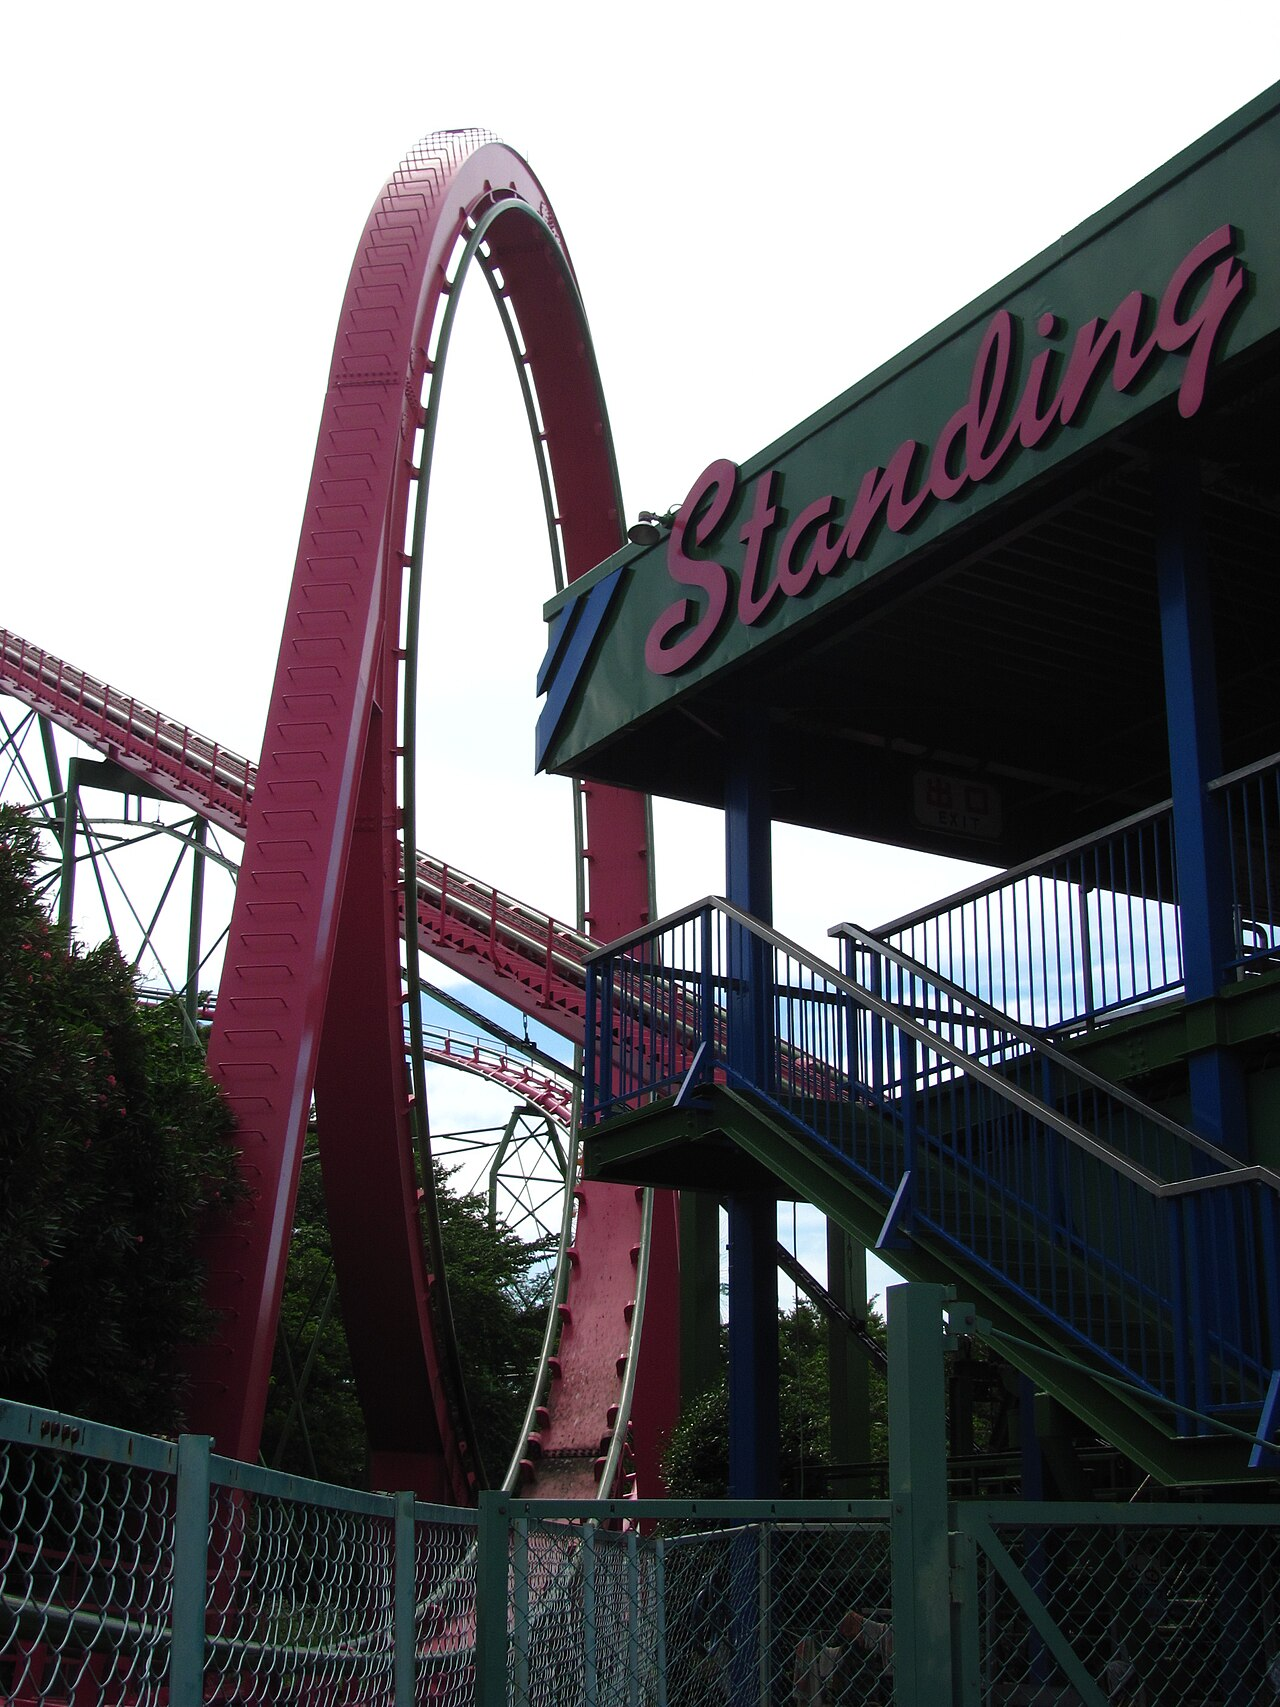
\includegraphics[width=0.38\linewidth]{images/book3/roller-coaster-loop.jpg}

{\small एक ऊर्ध्वाधर पाश (योमिउरीलैंड, टोक्यो): वृत्त नहीं, बल्कि अश्रु-बूँद के आकार का, ताकि वक्रता वहीं सबसे अधिक हो जहाँ चाल सबसे कम है, यानी शिखर पर --- यही सप्ताहांत समस्या की ज्यामिति है। छायाचित्र: जेरेमी थॉम्पसन, CC~BY~2.0।}
\end{omfigure}

\section{समस्या: झूला-रेलगाड़ी का पाश}

\begin{problem}[{सप्ताहांत समस्या --- कोई डिब्बी नब्बे किलोमीटर प्रति घंटा
की चाल से एक ऊर्ध्वाधर पाश में घुसती है: वह कहाँ धीमी पड़ती है, उसका त्वरण
किधर इंगित करता है, सवार कितने $g$ अनुभव करते हैं, और आधुनिक पाश वृत्त क्यों
नहीं होते}]
\label{pb:b1:point-kinematics:1}
कोई डिब्बी, जिसे बिंदु $M$ माना गया है, $R = \qty{10}{m}$ त्रिज्या और $C$
केंद्र वाले किसी ऊर्ध्वाधर वृत्तीय पाश पर दौड़ती है। उसकी स्थिति उस कोण
$\theta$ से दी जाती है जो $\vect{CM}$ और नीचे की ओर की ऊर्ध्वाधर के बीच
बनता है (तल पर $\theta =
0$ और शिखर पर $\pi$)। घर्षण नगण्य है, और चाल का नियम
(\cref{ch:b1:work-and-energy} में व्युत्पन्न) यह है:
\[
v^2 = v_0^2 - 2gR(1 - \cos\theta),
\]
जहाँ $v_0 = \qty{25}{m/s}$ तल पर की चाल है; $g = \qty{9.81}{m/s^2}$।

\medskip
\noindent\textbf{भाग I --- वृत्त पर शुद्धगतिकी।}
\begin{enumerate}
  \item $C$ पर केंद्रित ध्रुवीय निर्देशांकों में ($\vect e_r$ $C$ से $M$ की
        ओर), वृत्त पर की गति के लिए $\vect v$ और $\vect a$ लिखिए।
  \item फ्रेने सदिश $\vect T$ तथा $\vect N$ को $\vect e_r$ और
        $\vect e_\theta$ के पदों में पहचानिए, और \omterm{def:b1:point-kinematics:frenet}{वक्रता त्रिज्या} भी।
  \item शिखर पर, तथा पार्श्व बिंदुओं $\theta = \pi/2$ और $3\pi/2$ पर चाल
        निकालिए।
  \item चाल के नियम का समय के सापेक्ष अवकलन करके दिखाइए कि \omterm{thm:b1:point-kinematics:frenet}{स्पर्शरेखीय
        त्वरण} $a_T = -g\sin\theta$ है। ऊपर चढ़ते और नीचे उतरते समय उसके
        चिह्न की व्याख्या कीजिए।
  \item \omterm{thm:b1:point-kinematics:frenet}{अभिलंब त्वरण} $a_N(\theta)$ व्यक्त कीजिए और उसे तल पर, पार्श्वों पर
        तथा शिखर पर निकालिए।
  \item चारों बिंदुओं पर $\vect a$ का परिमाण दीजिए, और शिखर पर वह
        ऊर्ध्वाधर से जो कोण बनाता है वह भी।
  \item किन बिंदुओं पर $\vect a$, $\vect v$ पर लंब है? और किन पर समांतर?
\end{enumerate}

\medskip
\noindent\textbf{भाग II --- कोणीय दरें और समय।}
\begin{enumerate}[resume]
  \item $\dot\theta$ को $\theta$ के फलन के रूप में व्यक्त कीजिए और उसे तल
        पर तथा शिखर पर निकालिए।
  \item दिखाइए कि $\ddot\theta = -(g/R)\sin\theta$ (यही लोलक का समीकरण है)
        और उस पर टिप्पणी कीजिए।
  \item तुलना के लिए $R$ लंबाई के सरल लोलक के छोटे दोलनों का आवर्तकाल
        निकालिए (\cref{ex:b1:units-dimensions:pendulum} ने उसका रूप दे दिया
        था; $k = 2\pi$)।
  \item चारों संदर्भ बिंदुओं की चालों के औसत का प्रयोग करके पाश का एक चक्कर
        लगाने में लगे समय का आकलन कीजिए।
  \item डिब्बी के पटरी पर बने रहने के लिए शिखर पर न्यूनतम चाल $\sqrt{gR}$
        है (अगला अध्याय)। क्या वह पूरी होती है? न्यूनतम $v_0$ कितना चाहिए?
\end{enumerate}

\medskip
\noindent\textbf{भाग III --- सवार क्या अनुभव करते हैं।}
किसी सवार को अनुभव होता प्रति एकांक द्रव्यमान आभासी भार $\vect a - \vect g$
है (यहाँ स्वीकृत, \cref{ch:b1:newton-dynamics} में व्युत्पन्न); $g$ के
मात्रकों में उसका परिमाण ``$g$-भार'' कहलाता है।
\begin{enumerate}[resume]
  \item तल पर $g$-भार निकालिए।
  \item शिखर पर उसे निकालिए, और बताइए कि सवार किस ओर दबता है (सीट की ओर या
        बंधन की ओर)।
  \item पार्श्व बिंदुओं पर उसे निकालिए।
  \item सवार थोड़ी देर के लिए लगभग $4g$ सह लेते हैं। क्या यह पाश उत्तीर्ण
        होता है? समस्या कहाँ है?
  \item दिखाइए कि किसी वृत्तीय पाश में, जिसमें प्रवेश की चाल शिखर पार करने
        भर की ही हो (वहाँ आभासी भार शून्य), तल पर $g$-भार अनिवार्यतः $6g$
        होता है, चाहे $R$ कुछ भी हो।
\end{enumerate}

\medskip
\noindent\textbf{भाग IV --- क्लोथॉयड पाश।}
आधुनिक पाश ``अश्रु-बूँद'' जैसे होते हैं: \omterm{def:b1:point-kinematics:frenet}{वक्रता त्रिज्या} तल पर बड़ी और शिखर
पर छोटी होती है।
\begin{enumerate}[resume]
  \item $\vect a$ के फ्रेने रूप का प्रयोग करते हुए समझाइए कि पटरी के अनुदिश
        $\rho$ को बदलने से $a_N$ बदल जाता है, जबकि चाल का नियम (जो केवल
        ऊँचाई पर निर्भर है) नहीं बदलता।
  \item $\rho_{\text{तल}}$ ऐसा चुनिए कि तल पर $g$-भार $3g$ रहे, जब
        $v_0 = \qty{25}{m/s}$ हो।
  \item शिखर पर ऊँचाई अब भी तल से $2R = \qty{20}{m}$ ऊपर है।
        $\rho_{\text{शिखर}}$ ऐसा चुनिए कि वहाँ $g$-भार $1.5g$ हो।
  \item किसी क्लोथॉयड की वक्रता चाप लंबाई के समानुपाती होती है,
        $1/\rho = s/A^2$। ऐसे किसी प्रवेश-पथ पर, जब चाल लगभग अचर हो, $a_N$
        समय के साथ किस तरह बढ़ता है, और यह गरदन के लिए वृत्त से (जहाँ प्रवेश
        पर $a_N$ एकाएक कूद जाता है) अधिक कोमल क्यों है?
  \item परिणामी पाश का आकार गुणात्मक रूप से खींचिए और दो वाक्यों में सार
        दीजिए कि उसने वृत्त की जगह क्यों ले ली।
\end{enumerate}

\medskip
\noindent\textbf{भाग V --- भूमि से देखने पर।}
भूमि-तल पर रखा कोई \omterm{def:b1:optical-instruments:camera}{कैमरा}, जो पाश के तल में उसके केंद्र से \qty{50}{m} दूर है,
डिब्बी का पीछा करता है।
\begin{enumerate}[resume]
  \item जब डिब्बी शिखर पर है और \qty{15}{m/s} से क्षैतिज रूप से चल रही है,
        तब कैमरे को किस कोणीय दर (rad/s) से घूमना चाहिए? (कैमरे से ली गई
        ध्रुवीय निर्देशांक-व्यवस्था में।)
  \item अचर दर से घूमता \omterm{def:b1:optical-instruments:camera}{कैमरा} एकसमान \omterm{cor:b1:point-kinematics:circular}{वृत्तीय गति} का पीछा करने में खराब
        क्यों रहता है?
  \item इस पाश से मिले अध्याय के पाठ का सार दीजिए: किस
        निर्देशांक-व्यवस्था ने किस प्रश्न का उत्तर दिया।
\end{enumerate}
\end{problem}
